% !TEX program = xelatex
% Отчёт по ДЗ2 (генерация кода). Сборка: latexmk -xelatex report.tex
\documentclass[11pt,a4paper]{article}
\usepackage{fontspec}
\defaultfontfeatures{Ligatures=TeX}
\usepackage{polyglossia}
\setdefaultlanguage{russian}
\setotherlanguage{english}
\setmainfont{cmunrm.otf}[BoldFont=cmunbx.otf,ItalicFont=cmunti.otf,BoldItalicFont=cmunbi.otf]
\setsansfont{cmunss.otf}[BoldFont=cmunsx.otf,ItalicFont=cmunsi.otf,BoldItalicFont=cmunso.otf]
\setmonofont{cmuntt.otf}[BoldFont=cmuntb.otf,ItalicFont=cmunit.otf]
\newfontfamily\cyrillicfont{cmunrm.otf}[BoldFont=cmunbx.otf,ItalicFont=cmunti.otf,BoldItalicFont=cmunbi.otf]
\newfontfamily\cyrillicfontsf{cmunss.otf}[BoldFont=cmunsx.otf,ItalicFont=cmunsi.otf,BoldItalicFont=cmunso.otf]
\newfontfamily\cyrillicfonttt{cmuntt.otf}[BoldFont=cmuntb.otf,ItalicFont=cmunit.otf]
\usepackage[a4paper,margin=2cm]{geometry}
\usepackage{graphicx,booktabs,tabularx,array,enumitem,xcolor,xspace,icomma,fancyvrb}
\usepackage[most]{tcolorbox}
\usepackage{tikz}
\usetikzlibrary{arrows.meta,positioning,fit,backgrounds}
\usepackage{hyperref}
\hypersetup{colorlinks=true,linkcolor=black,citecolor=black,urlcolor=blue!55!black}
\usepackage{url}
\usepackage{caption}
\usepackage{float}
\captionsetup{font=small,labelfont=bf}
\setlist{itemsep=1pt,topsep=3pt,leftmargin=*}
\setlength{\parskip}{3pt}
\graphicspath{{figures/}}

% Блок для собственных размышлений автора. Серый текст внутри — подсказка, её нужно заменить своим текстом.
\newtcolorbox{mythoughts}{colback=yellow!8,colframe=orange!60!black,boxrule=.5pt,arc=2pt,
  title=Мои мысли,fonttitle=\bfseries\small,left=4pt,right=4pt,top=2pt,bottom=2pt}
\newcommand{\hint}[1]{{\color{gray}\itshape #1}}
\newcommand{\pp}{п.\,п.\xspace}
% Публичный репозиторий и датасет весов.
\newcommand{\repourl}{https://github.com/thisariv/hse-nlp-hw2-code-generation}
\newcommand{\repo}{\url{\repourl}}
\newcommand{\weightsurl}{https://www.kaggle.com/datasets/thisarivson/nlp-hw02-final-weights}
% Путь внутри репозитория: моноширинный, с переносами, кликабельный (ведёт в GitHub).
\newcommand{\file}[1]{\href{\repourl/tree/main/#1}{\path{#1}}}

\title{\textbf{Генерация кода маленьким Transformer'ом}}
\author{Владимир Родин \\ \small ДЗ2 по NLP, НИУ ВШЭ, 2026}
\date{}

\begin{document}
\maketitle
\vspace{-1.5em}

%======================================================================
\section*{Вступление + описание итоговой архитектуры}

\textbf{Вступление.} Когда я узнал, что у нас будет домашнее задание с лидербордом и с использованием агентов, я очень обрадовался, ведь когда есть лидерборд лично у меня просыпается соревановательный дух, а разрешение на использование агентов помогает попробовать много разного и в итоге найти оптимальное решение. Мое решение этого дз скорее не про супер иновационное решение, а про грамотную работу с агентами, как мне кажется в современном мире это иногда даже важнее каких-то теоретических знаний в области. В первом разделе я расскажу про итоговую архитектуру решения, а затем будет долгий рассказ в хронологическом порядке как мы к этому пришли.

\textbf{Задача.} Обучить с нуля encoder-decoder Transformer, который по текстовой задаче из датасета TinyGSM пишет функцию \texttt{solve()} на Python. Ответ засчитывается, если код при исполнении выдаёт правильное число. Все 1919 тестовых задач нужно решить не дольше чем за 180 секунд на одной видеокарте T4.

\textbf{Результат.} \textbf{80,10\%} на публичном лидерборде (1--2 место на момент 21ое октября). Финальное решение~--- ансамбль из трёх моделей ($\approx$100M + 54M + 54M параметров), который голосует по результатам исполнения кода и укладывается в $\approx$123 с.

\textbf{Код и файлы.} Весь код, ноутбуки и записи экспериментов лежат в публичном репозитории \repo. Ниже пути указаны относительно корня репозитория. Главное для проверки: \file{submission/inference.ipynb} (финальный ноутбук), \file{submission/README.md} (как запустить) и \file{submission/code/hw2_codegen/} (чистый код инференса и обучения).

\begin{figure}[h]
  \centering
  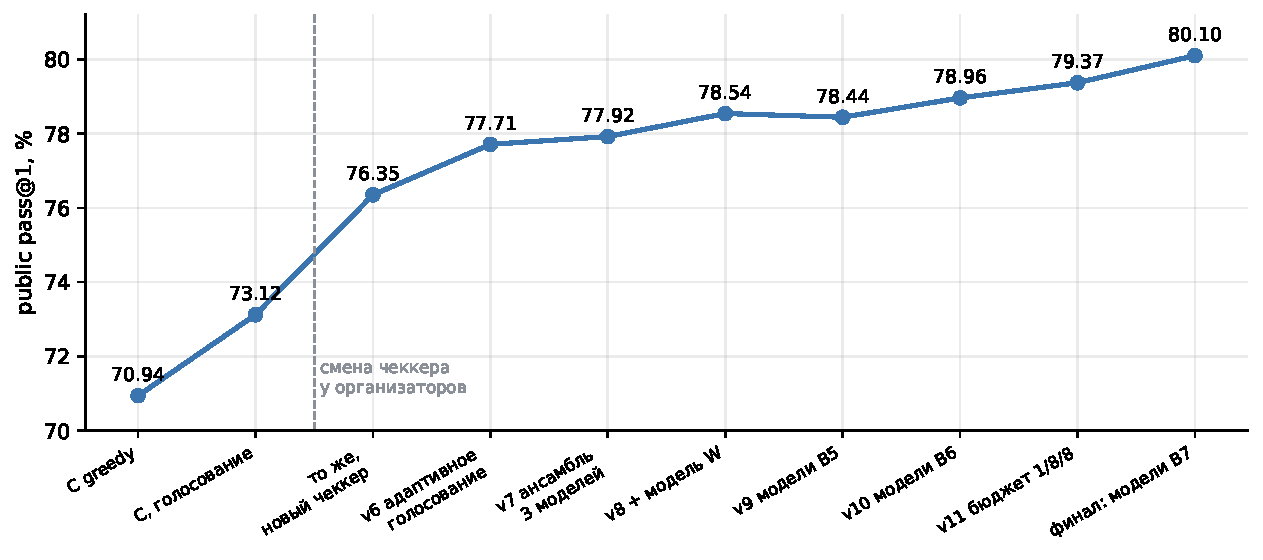
\includegraphics[width=\linewidth]{leaderboard}
  \vspace{-1.5em}
  \caption{Публичный лидерборд по нашим посылкам. Каждая точка~--- одно улучшение инференса или моделей.}
  \label{fig:lb}
\end{figure}

\begin{figure}[h]
  \centering
  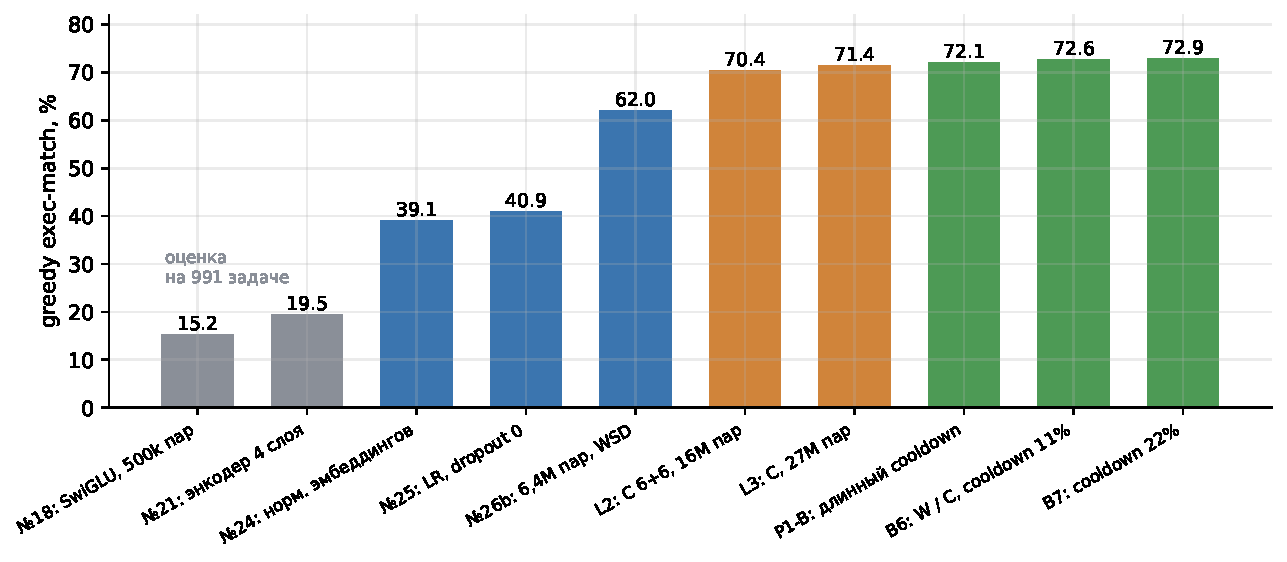
\includegraphics[width=\linewidth]{single_model_path}
  \vspace{-1.5em}
  \caption{Как росло качество одной модели (greedy, без голосования): от эксперимента №18 этапа 1 до финальных моделей этапа 2.}
  \label{fig:path}
\end{figure}

\subsection*{Описание итоговой архитектуры}

Решение состоит из четырёх частей: данные и их представление, три модели, рецепт обучения и инференс с голосованием.

\paragraph{Данные.} Используется только разрешённый датасет \texttt{SlavaYus/tinysms\_qa\_12m}. Мы отбросили пары, у которых вопрос длиннее 512 байт или код не короче 512 байт в UTF-8. Ещё убрали пары, чей эталонный код при исполнении не даёт конечного числа, и вопросы, совпадающие с тестом. Хешем (seed 42) отложили 4096 задач для валидации (\emph{heldout4k}); её делим пополам на \emph{tune} и \emph{eval} по 2048. Осталось \textbf{9\,725\,737 пар} для обучения; текстовые дубли не удаляли. Новых данных и новых таргетов не создавали: меняется только запись того же кода.

\paragraph{Представление кода.} Почти все программы начинаются с одинаковой «шапки» и заканчиваются строками \texttt{result = …} / \texttt{return result}. Мы убираем эти повторяющиеся куски обратимым преобразованием. Модель генерирует только смысловую часть, а перед исполнением код восстанавливается.

\begin{center}
\begin{minipage}{.46\linewidth}\small\textbf{Исходный код}
\begin{Verbatim}[fontsize=\footnotesize,frame=single]
def solve() -> int:
    perimeter = 64
    side = perimeter / 4
    result = side
    return result
\end{Verbatim}
\end{minipage}\hfill
\begin{minipage}{.46\linewidth}\small\textbf{Что генерирует модель}
\begin{Verbatim}[fontsize=\footnotesize,frame=single]
<|header_tail|>
    perimeter = 64
    side = perimeter / 4
    side
\end{Verbatim}
\end{minipage}
\end{center}

\paragraph{Токенизатор.} Собственный BPE на 8189 токенов в стиле Qwen: каждая цифра~--- отдельный токен, поэтому числа всегда разбиваются одинаково. Ещё 3 служебных токена режима записи и PAD/BOS/EOS~--- всего \textbf{8195} токенов. Ответ ограничен 512 токенами.

\paragraph{Модели.} Все три модели~--- обычные encoder-decoder Transformer'ы (\texttt{nn.\allowbreak Transformer} из PyTorch) с одинаковой схемой слоя: Pre-LN (LayerNorm перед блоком), SwiGLU вместо обычного FFN, обученные позиционные эмбеддинги (до 2048 позиций), отдельная (не связанная с эмбеддингами) выходная голова, dropout 0. Эмбеддинги токенов инициализируются нормированными: веса делятся на $\sqrt{d}$, а на входе умножаются на $\sqrt{d}$ (см. эксперимент №24). Код~--- \file{submission/code/hw2_codegen/model.py}.

\begin{center}\small
\begin{tabular}{lcc}
\toprule
& \textbf{C} (C-long2x B7, P1-B) & \textbf{W} (W B7) \\
\midrule
Слоёв энкодер + декодер & 6 + 6 & 6 + 6 \\
$d_\text{model}$ / головы attention & 512 / 8 & 768 / 12 \\
Скрытый размер SwiGLU & 1368 & 2048 \\
QK-нормализация (LayerNorm на $q$ и $k$ в каждой голове) & нет & да \\
Параметров & $\approx$54M & $\approx$99M \\
\bottomrule
\end{tabular}
\end{center}

\paragraph{Обучение.} Общий рецепт для всех моделей (\file{submission/code/hw2_codegen/train.py}):
\begin{itemize}
  \item AdamW (betas 0,9/0,999), weight decay 0,01, клиппинг градиента по норме 1,0;
  \item смешанная точность FP16 + GradScaler (начальный масштаб 1024);
  \item эффективный батч 128 пар (2 микробатча по 64); группировка по длине: примеры сортируются локально блоками по 4096 и режутся на батчи, порядок батчей перемешан;
  \item функция потерь~--- кросс-энтропия по токенам ответа; для W дополнительно z-loss с весом $10^{-4}$ (штраф за рост $\log\sum e^{\text{logit}}$, стабилизирует FP16);
  \item порядок данных \emph{long2x}: длинные примеры встречаются в эпохе дважды (у C-long2x и W);
  \item расписание LR \textbf{WSD} (warmup–stable–decay): короткий линейный warmup, затем долгий \emph{постоянный} LR, затем отдельный участок охлаждения до нуля по форме $\eta_j=\eta_0\bigl(1-\sqrt{j/N}\bigr)$, где $\eta_0$~--- постоянный LR, $j$~--- номер шага охлаждения, $N$~--- его длина.
\end{itemize}
Плюс WSD в том, что из любой точки постоянного участка можно сделать отдельное охлаждение, получить готовую модель и продолжить основное обучение дальше.

\begin{center}\small
\begin{tabularx}{\linewidth}{lccc>{\raggedright\arraybackslash}X}
\toprule
Модель & Warmup & Постоянный LR & Пар в основной части & Охлаждение \\
\midrule
W B7 & 2000 шагов & $6\cdot10^{-4}$ & 19,8M & $1-\sqrt{t}$, 33\,000 шагов \\
C-long2x B7 & 1000 шагов & $1{,}5\cdot10^{-3}$ & 37,6M & $1-\sqrt{t}$, 65\,800 шагов \\
P1-B & 1000 шагов & $1{,}5\cdot10^{-3}$ & 26,8M & $1-\sqrt{t}$, 31\,372 шага + loss truncation 10\% \\
\bottomrule
\end{tabularx}
\end{center}

Loss truncation у P1-B: в каждом батче отбрасываются 10\% примеров с самой большой ошибкой (отдельно по корзинам длины). Обучение шло сессиями по 10--11 часов на Kaggle (2$\times$T4); между сессиями сохранялось полное состояние (веса, AdamW, GradScaler, RNG, позиция в данных), поэтому продолжение было бит-в-бит.

\paragraph{Инференс.} Схема на рис.~\ref{fig:final}. Для каждой задачи:
\begin{enumerate}
  \item \textbf{greedy} от модели-якоря W B7;
  \item \textbf{этап 1}: по одному сэмплу ($T=0{,}7$) от W B7, C-long2x B7 и P1-B;
  \item каждый кандидат \textbf{исполняется} в песочнице (лимит 3\,с, 768\,МБ памяти, отдельный процесс); если все 4 числа совпали ($|a-b|\le10^{-6}$), это ответ~--- так решаются \textbf{62\%} задач;
  \item иначе \textbf{этап 2}: досэмплируем до 8 сэмплов от C-long2x B7 и от P1-B (всего до 17 сэмплов плюс greedy);
  \item \textbf{голосование}: кандидаты группируются по численному ответу, побеждает самая большая группа. При равенстве~--- группа, где есть greedy, затем~--- с наибольшим средним log-prob. Победивший код ещё раз исполняется для проверки.
\end{enumerate}

\begin{figure}[h]
\centering
\begin{tikzpicture}[node distance=4mm and 6mm, every node/.style={font=\small},
  box/.style={draw,rounded corners,align=center,minimum height=8mm,fill=#1!10}, box/.default=blue,
  arr/.style={-{Stealth[length=2mm]},thick}]
\node[box=gray] (q) {задача\\(текст)};
\node[box, right=of q] (g) {greedy\\W B7};
\node[box, right=of g] (s1) {этап 1: по 1 сэмплу\\W B7, C B7, P1-B};
\node[box=green, right=of s1, yshift=6mm] (ok) {все 4 ответа\\совпали → готово};
\node[box=orange, right=of s1, yshift=-8mm] (s2) {этап 2: до 8 сэмплов\\C B7 и P1-B};
\node[box=red, below=of s1, yshift=-4mm] (ex) {исполнение кода\\в песочнице};
\node[box=green, left=of ex] (v) {голосование\\по числу → ответ};
\draw[arr] (q) -- (g); \draw[arr] (g) -- (s1);
\draw[arr] (s1) -- (ok); \draw[arr] (s1) -- (s2);
\draw[arr] (s2) |- (ex); \draw[arr] (ex) -- (v);
\end{tikzpicture}
\caption{Финальный инференс. Каждое решение исполняется; побеждает самый частый численный ответ.}
\label{fig:final}
\end{figure}

\paragraph{Быстрый декодер.} Обычная генерация батчем устроена так: берём $N$ задач и генерируем ответы токен за токеном, пока не закончат \emph{все}. Короткие ответы заканчиваются рано, но их строки остаются в батче, и GPU продолжает считать для них пустые токены (рис.~\ref{fig:decoder}, слева). Кроме того, после каждого шага программа спрашивает GPU «все ли закончили?» и ждёт ответа, а пока она ждёт, GPU простаивает. Для голосования нужно в $\approx$8 раз больше генераций, чем для greedy, поэтому такие потери становятся критичными. Наш декодер (\file{submission/code/hw2_codegen/decode.py}) устроен иначе:
\begin{itemize}
  \item \textbf{KV-кеш}: ключи и значения уже сгенерированных токенов не пересчитываются (№07: в 6 раз быстрее);
  \item \textbf{батч по бюджету строк}: одновременно генерируется фиксированное число последовательностей (640), куда кладутся и разные задачи, и сэмплы одной задачи; задачи заранее отсортированы по длине вопроса;
  \item \textbf{уплотнение}: когда закончила четверть строк, законченные выкидываются, и батч становится меньше (рис.~\ref{fig:decoder}, справа);
  \item \textbf{проверка конца раз в 32 шага}, а не на каждом шаге, без ожидания GPU;
  \item \textbf{общий энкодер}: вопрос кодируется один раз, и ключи/значения cross-attention общие для всех сэмплов этой задачи;
  \item \textbf{сэмплирование одним действием на GPU}: к log-вероятностям добавляется случайный шум и берётся максимум (трюк «exponential race», эквивалентный обычному сэмплированию из softmax);
  \item \textbf{GPU и CPU работают одновременно}: пока GPU генерирует следующий батч, 4 процесса на CPU уже исполняют готовый код.
\end{itemize}
Профилирование и эти изменения ускорили greedy в 1,7--1,9 раза, а сэмплирование~--- в 1,3--1,6 раза (\file{work/notes/decode-speed.md}). В итоге голосование, которое в первой версии занимало 493\,с (№27), стало укладываться в $\approx$120\,с вместе с greedy и исполнением. Есть и защитный таймер: если к 160\,с генерация не закончена, оставшимся задачам отдаётся greedy-ответ (в финальных прогонах он не срабатывал). Распределение времени~--- на рис.~\ref{fig:time}.

\begin{figure}[h]
\centering
\begin{tikzpicture}[x=3.2mm,y=4mm,every node/.style={font=\scriptsize}]
% left: naive batch
\node[anchor=west,font=\small\bfseries] at (0,5.4) {обычный батч};
\foreach \len/\y in {7/4,16/3,10/2,4/1}{
  \fill[blue!45] (0,\y-.4) rectangle (\len,\y+.4);
  \fill[gray!25] (\len,\y-.4) rectangle (16,\y+.4);
}
\draw[->] (0,0.2) -- (17,0.2) node[right] {шаги};
\node[anchor=north west,text width=52mm] at (0,-.3) {серым~--- строки уже закончили, но GPU продолжает их считать};
% right: our decoder
\begin{scope}[xshift=68mm]
\node[anchor=west,font=\small\bfseries] at (0,5.4) {наш декодер};
\fill[blue!45] (0,3.6) rectangle (7,4.4);  \fill[orange!60] (7,3.6) rectangle (15,4.4);
\fill[blue!45] (0,2.6) rectangle (16,3.4);
\fill[blue!45] (0,1.6) rectangle (10,2.4); \fill[orange!60] (10,1.6) rectangle (14,2.4);
\fill[blue!45] (0,0.6) rectangle (4,1.4);  \fill[orange!60] (4,0.6) rectangle (12,1.4);
\draw[->] (0,0.2) -- (17,0.2) node[right] {шаги};
\node[anchor=north west,text width=52mm] at (0,-.3) {законченные строки выкидываются, на их место встают новые задачи (оранжевые)};
\end{scope}
\end{tikzpicture}
\caption{Идея быстрого декодера: GPU не тратит время на уже законченные ответы.}
\label{fig:decoder}
\end{figure}

\begin{figure}[h]
  \centering
  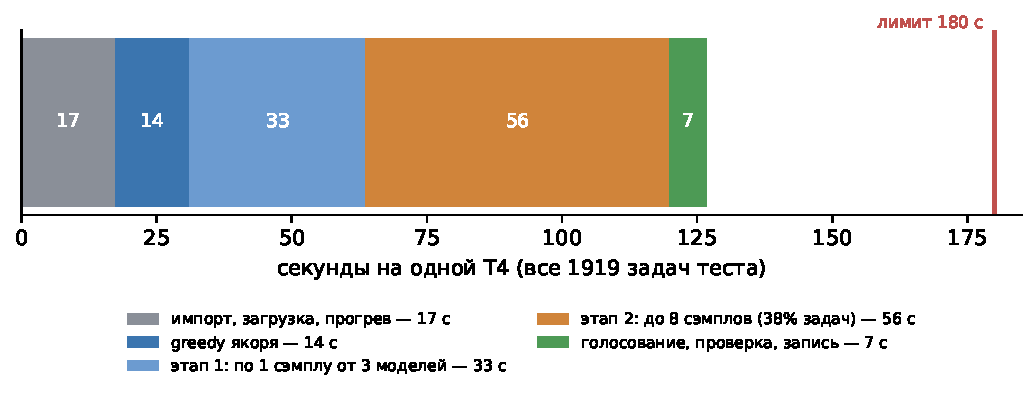
\includegraphics[width=.85\linewidth]{time_budget}
  \vspace{-.8em}
  \caption{На что уходит время на T4 (финальный прогон: 122,7\,с, пик памяти 11,1\,ГБ).}
  \label{fig:time}
\end{figure}

\begin{center}\small
\begin{tabular}{lcccc}
\toprule
Модель & Greedy, \% (heldout4k) & Голосование 8 сэмплов (tune) & & \\
\midrule
W B7 (якорь) & 72,92 & 74,5 \\
C-long2x B7 & 72,85 & 74,2 \\
P1-B & 72,07 & 74,3 \\
\midrule
\multicolumn{2}{l}{\textbf{Ансамбль} (tune, 2048 задач, свежий прогон)} & \textbf{76,2} \\
\bottomrule
\end{tabular}
\end{center}

\textbf{Воспроизводимость.} Метод сэмплирует, а порядок досэмплирования на GPU зависит от тайминга. Поэтому два запуска дают немного разные ответы.

%======================================================================
\section{Этап 1}

Теперь расскажу более подробно, что я делал. Я не хотел сразу обучать что-то большое с какими-то модификациями, поэтому я решил начать с самой базы, на это этапе я работал с codex gpt 6.1 sol max effort. Мы начали с самой простой модели: байтовый Transformer 2+2 слоя, $d=128$, 1,25M параметров, 512 пар и 200 шагов обучения (\\ \file{work/notebooks/01-baseline-byte-512-pairs-200-steps.ipynb}). Модель ещё не умела генерировать осмысленный код. Тогда мы проверили сам пайплайн: сможет ли модель хотя бы \textbf{запомнить 16 примеров}. Смогла~--- все 16 точно к шагу 2250 (ноутбуки 03--04). Значит, код обучения и генерации работает, и можно масштабироваться.

Дальше мы шли маленькими шагами: в каждом ноутбуке менялась одна вещь, а модель была маленькой, поэтому один эксперимент занимал минуты или десятки минут в Colab. Так за неделю получилось провести 26 экспериментов (табл.~\ref{tab:phase1}). Все ноутбуки лежат в \file{work/notebooks/}, их результаты с выводами~--- в \file{work/results/}, а разбор каждого шага~--- в \file{work/notes/}.

\begin{table}[tbp]
\centering\small
\caption{Эксперименты этапа 1. Номер~--- префикс ноутбука в \texttt{work/notebooks/}.}
\label{tab:phase1}
\begin{tabularx}{\linewidth}{l>{\raggedright\arraybackslash}X>{\raggedright\arraybackslash}X}
\toprule
№ & Что меняли & Что получилось \\
\midrule
01--02 & байтовый Transformer 2+2, $d=128$; 200\,→\,2000 шагов & код почти не компилируется (3/64 синтаксически верных) \\
03--04 & запомнить 16 пар & 16/16 точно к шагу 2250~--- пайплайн рабочий \\
05--06 & 20k пар, 10k\,→\,50k шагов & форма программы лучше, правильность слабая \\
07 & KV-кеш при генерации & инференс 370\,→\,61\,с (в 6 раз), ответы совпали побитно \\
08 & BPE-токенизатор на 4k & синтаксически верных 57\,→\,95\%, ошибки отступов 754\,→\,2 \\
09--12 & ширина 256, cosine LR, 100k пар, warmup & ширина без других изменений ухудшила; данные и расписание помогли loss \\
13--15 & Pre-LN, обучение до 100k шагов, SwiGLU & стабильнее и лучше: численные совпадения 104\,→\,117\,→\,123 из 888 \\
16 & кеш BPE, AMP FP16 при батче 8 & кеш $-6\%$ времени шага; FP16 на маленьком батче медленнее \\
17--18 & 500k пар & новая база: 15\% задач с правильным ответом (151/991) \\
19--22 & BPE 8k с раздельными цифрами, 4 слоя в декодере/энкодере & до 19\% (193/991), различия на грани шума \\
23 & батч 128, FP16, группировка по длине & обучение быстрее в \textbf{5,7 раза}; инференс 71\,→\,16\,с \\
24 & нормированная инициализация эмбеддингов & \textbf{20,0\,→\,39,1\%}~--- самый большой скачок \\
25 & LR 0,003, dropout 0 & 40,9\% \\
26a--b & 7M пар с проверенным исполнением, WSD & 46,1\,→\,54,0\,→\,62,0\% при росте данных до 6,4M пар \\
\bottomrule
\end{tabularx}
\end{table}

\textbf{Что поняли на этом этапе.} Сильнее всего помогли не архитектурные трюки, а «скучные» вещи: скорость обучения, нормированные эмбеддинги и большой объём данных.

%======================================================================
\section{Этап 2}

В какой-то момент я понял, что пора масштабироваться и поэтому перешел на другую схему взаимодействия с агентами (я уже так работал над разными своими проектиками и такая схема мне нравилась). На этот раз я общался с claude opus 5.5 как с оркестратором, важно чтобы он не тратил лимиты и самое важное контекст на написание кода, копания в логах и тд, благодаря этому claude не компактил контекст во время каждой сессии, что регулярно происходит если работать с кодекс даже на самом маленьком проекте. Для того чтобы claude не засорял контекст всю грязную работу делает codex, для этого claude может запускать codex в терминале через «codex exec». Дальше мы использовали много сессий codex как агента который пишет код, ревьюит код, анализирует результаты, проводит ресерч и тд. Может показаться, что для этого нужны какие-то супер подписки, но это не так, у меня самые базовые 20\$ подписки на клод и гпт и этого вполне хватает. Вот маленькая нейрослопная схема:

\begin{figure}[H]
\centering
\begin{tikzpicture}[node distance=6mm and 7mm, every node/.style={font=\small},
  box/.style={draw,rounded corners,align=center,minimum height=9mm,text width=27mm,fill=#1!10}, box/.default=blue,
  arr/.style={-{Stealth[length=2mm]},thick}]
\node[box=orange] (me) {\textbf{Я}\\ направление,\\ решения, ресурсы};
\node[box=blue, right=of me] (orch) {\textbf{Оркестратор}\\ (Claude): план,\\ анализ, промпты};
\node[box=green, right=of orch] (exec) {\textbf{Исполнитель}\\ (Codex): код,\\ CPU-тесты};
\node[box=red, right=of exec] (rev) {\textbf{Ревьюер}\\ (другой Codex):\\ ревью, смоук};
\node[box=gray, below=of rev] (kg) {\textbf{Kaggle}\\ 2$\times$T4};
\node[box=green, below=of exec] (an) {\textbf{Аналитик}\\ (Codex): разбор\\ результатов};
\node[box=gray, below=of orch] (git) {\textbf{Git + заметки}\\ каждый шаг\\ записан};
\draw[arr] (me) -- (orch);
\draw[arr] (orch) -- (exec);
\draw[arr] (exec) -- (rev);
\draw[arr] (rev) -- node[right,font=\scriptsize]{запуск} (kg);
\draw[arr] (kg) -- node[above,font=\scriptsize]{вотчер} (an);
\draw[arr] (an) -- (git);
\draw[arr] (git) -| node[pos=.25,above,font=\scriptsize]{итоги} (me);
\end{tikzpicture}
\caption{Цикл одного эксперимента}
\label{fig:agents}
\end{figure}

\textbf{Оркестратор и команда агентов.} Обучение стало долгим (по 10 часов), и цена ошибки выросла. Поэтому работа разделилась на роли (рис.~\ref{fig:agents}). Оркестратор пишет задание для Codex в виде промпта: контекст, что сделать, какие проверки пройти, что записать. Исполнитель готовит код и проверяет его на CPU. Другой, независимый Codex делает ревью и короткий смоук на GPU, и только после этого запускает долгую сессию. Когда сессия на Kaggle заканчивается, скрипт-вотчер скачивает результаты и запускает Codex-аналитика. Оркестратор читает короткий итог, коммитит и приносит мне решение.

Для начала я определил несколько правил которые надо было соблюдать, чтобы эксперименты не превратились в кашу и было понятно что к чему
\begin{itemize}
  \item \textbf{Одно изменение за раз} и заранее записанная гипотеза.
  \item \textbf{Независимое ревью} перед каждым длинным запуском: код писал один агент, проверял другой. Затем \textbf{смоук}~--- короткий прогон на GPU на 10 минут.
  \item \textbf{Честная проверка}: выбираем вариант на одной выборке, подтверждаем на другой. Критерий успеха записываем \emph{до} того, как смотрим на результат.
  \item \textbf{Всё в Git}: план, ревью, результаты и выводы каждого шага лежат рядом с кодом (\file{work/notes/}: \texttt{*-plan.md}, \texttt{*-review.md}, \texttt{*-results.md}).
\end{itemize}

Дальше~--- эксперименты этого этапа по порядку. Код запусков на Kaggle~--- в \file{work/kaggle/} (сборщики \texttt{build\_*.py}, исходники \file{work/kaggle/src/}), скрипты анализа~--- в \file{work/research/}.

\subsection{Разведка и длинное обучение модели C}
Сначала мы провели три короткие разведочные сессии на Kaggle (S1--S3, эксперименты №27--32):
\begin{itemize}
  \item \textbf{S1~--- голосование.} Голосование по 32 сэмплам дало 66,6\% против 62,0\% у greedy, но заняло 493\,с вместо 180 (\file{work/notes/27-execution-voting-s1-results.md}). Стало понятно, что голосование~--- главный резерв, но нужен быстрый инференс.
  \item \textbf{S2~--- ёмкость.} Модель побольше (B) при равном времени обучения оказалась не лучше базовой: 61,4\% против 62,0\% (\file{work/notes/29m-28b-capacity-s2-results.md}).
  \item \textbf{S3~--- представление кода.} Компактная запись кода дала на 15\% больше пар в секунду при том же качестве; её приняли как стандарт (\file{work/notes/s3-representations-results.md}).
\end{itemize}

Затем модель C (6+6, $d=512$) учили длинными сессиями по 10 часов (\\ \file{work/notes/l1-long-training.md}, \texttt{l2-results.md}, \texttt{l3-results.md}). В L1 обучили C с нуля ($\approx$6M пар), в L2 и L3 продолжали две ветки из одной точки: обычный порядок данных (C-main) и порядок, где длинные примеры встречаются дважды (C-long2x). Каждые несколько часов мы делали короткое охлаждение (15 или 50 минут) и мерили качество (рис.~\ref{fig:curves}). C-long2x оказалась немного лучше: после L3 \textbf{70,8\%} (C-main) и \textbf{71,4\%} (C-long2x) на 27M парах. Но рост почти остановился: последние 10 часов дали меньше 1\,\pp

Параллельно мы строили инференс. Первые посылки: одна модель greedy~--- 70,9\%, голосование по 4+4 сэмпла двух моделей~--- 73,1\%. Затем организаторы поправили чеккер, и та же посылка получила 76,4\%. Дальше было несколько версий инференса (\file{work/notes/final-inference.md}):
\begin{itemize}
  \item в v1 нашлась ошибка путей к данным Kaggle, в v2~--- защитный таймер откатывал \emph{все} ответы к greedy, а батчи считались по задачам, поэтому 2 сэмпла стоили столько же, сколько 4;
  \item v5 перешла на батчи по бюджету строк и стала сначала досэмплировать самые спорные задачи;
  \item v6~--- адаптивное голосование (greedy, затем дополнительные сэмплы только при разногласии): \textbf{77,7\%};
  \item v7~--- ансамбль трёх моделей C (C-main, C-long2x, P1-B): \textbf{77,9\%}.
\end{itemize}

\begin{figure}[h]
  \centering
  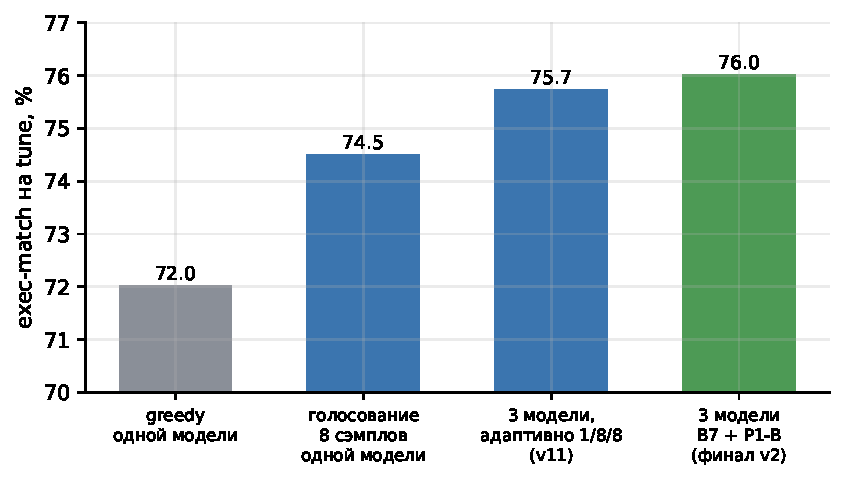
\includegraphics[width=.62\linewidth]{voting}
  \vspace{-.6em}
  \caption{Что даёт голосование (tune, 2048 задач): одна модель greedy → голосование 8 сэмплов → ансамбль трёх моделей.}
  \label{fig:voting}
\end{figure}

\subsection{Попытки пробить плато модели C}
Мы проверили несколько гипотез, почему C перестала расти:
\begin{itemize}
  \item \textbf{Переобучение?} Нет. На трейне и на отложенной выборке CE отличается всего на 0,047, точность по токенам~--- 93,6 и 92,4\%, и разрыв не растёт (\file{work/notes/overfit-check.md}). Модель не запоминает трейн, а упирается во что-то другое.
  \item \textbf{Шум в разметке} (D1). Если в датасете есть пары с ошибочным эталоном, их можно найти по разногласию: несколько моделей решают задачу, и если все они уверенно расходятся с эталоном, эталон, скорее всего, неверный. Проверили это на повторяющихся вопросах, где правильный ответ известен по большинству: среди 886 кандидатов модели совпали с ним лишь в 14\% случаев. Такой фильтр выкидывал бы в основном хорошие примеры, поэтому его не применили (\file{work/notes/d1-results.md}).
  \item \textbf{Глубже энкодер} (R1). Энкодер вырастили с 6 до 12 слоёв «с сохранением функции»: новые слои инициализировались так, что модель сначала выдаёт то же самое, а потом доучивается. За 10 часов~--- +0,15\,\pp, в пределах шума (\file{work/notes/r1-results.md}).
  \item \textbf{Длинное охлаждение} (P1). Из конца L3 сделали две ветки: охлаждение 3,6 часа вместо 50 минут по форме $1-\sqrt{t}$ (P1-A) и то же самое с loss truncation (P1-B). P1-A дала +0,3\,\pp, P1-B~--- \textbf{+0,7\,\pp} (72,07\%), так появилась модель P1-B (\file{work/notes/p1-results.md}). Оба прироста были на грани шума, и тогда мы ещё не поняли, насколько важно охлаждение.
\end{itemize}

\subsection{Модель побольше: W с QK-нормализацией}
По закону Chinchilla (Hoffmann et al., 2022) для фиксированного объёма вычислений есть оптимальный размер модели: слишком маленькая быстро «насыщается», слишком большая не успевает выучиться. По нашей оценке, модель C была мала: при нашем объёме обучения оптимум~--- $\approx$90--130M параметров (\file{work/notes/architecture-decision.md}). Мы замерили на T4 скорость обучения и генерации для 13 форм модели (разная глубина и ширина) и выбрали W (6+6, $d=768$): сэмпл в 1,35 раза дороже, чем у C, и инференс ансамбля всё ещё укладывается в лимит.

\textbf{B1: первая попытка провалилась.} Две большие модели с нуля (W 6+6 и E 8+4, обе $d=768$) учились 10,5 часа, но обучение периодически расходилось: loss резко рос, появлялись NaN. Автоматическое восстановление откатывало модель и дважды уменьшало LR, и в итоге обе модели отстали от C.

\textbf{B2: QK-нормализация.} Причина таких срывов в больших Transformer'ах~--- рост логитов attention: скалярные произведения запросов и ключей становятся огромными, softmax «залипает», а в FP16 случается переполнение. Мы добавили три вещи: LayerNorm на запросах и ключах в каждой голове (QK-norm), z-loss с весом $10^{-4}$ и warmup 2000 шагов. Обучение стало стабильным, и при одинаковом числе пар (3,1M) W обогнала C: 64,3\% против 62,9\% (\file{work/notes/b2-results.md}).

\textbf{B3--B5: продолжение W.} В B3 продолжили две ветки с разным LR: $6\cdot10^{-4}$ оказался лучше $10^{-3}$ (70,4 против 69,6\% с 50-минутным охлаждением), дальше шли с ним. В B4 вторая ветка пробовала loss truncation в основном обучении~--- она хуже на 0,95\,п.\,п. В B5 ещё 9 часов обучения W дали всего +0,05\,\pp (70,95\% на 19,8M парах), а продолжение C-long2x до 37,6M пар~--- даже $-0,24$\,\pp При равном числе пар W была на 1,5--2\,\pp лучше C, но обе модели упёрлись примерно в 71\%.

\begin{figure}[h]
  \centering
  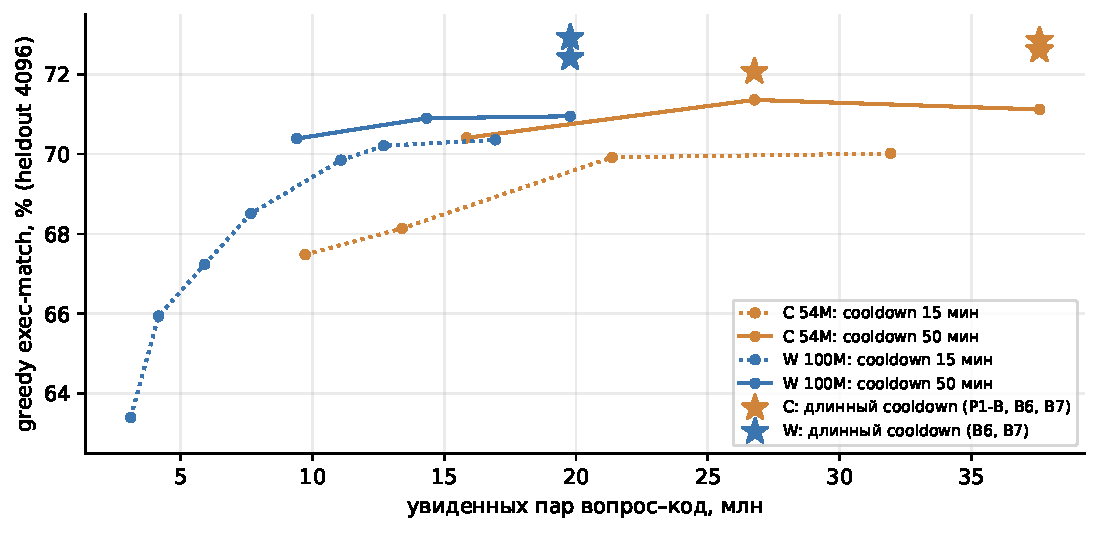
\includegraphics[width=.8\linewidth]{learning_curves}
  \vspace{-.8em}
  \caption{Кривые обучения C и W. Точки~--- промежуточные модели с коротким охлаждением; звёзды~--- те же модели после длинного охлаждения.}
  \label{fig:curves}
\end{figure}

\subsection{Главная находка: длинное охлаждение}
Почему охлаждение вообще помогает? При большом постоянном LR веса модели «прыгают» по дну долины функции потерь и не опускаются в самую низкую точку. Охлаждение плавно уменьшает шаг, и модель «оседает». Наше плато оказалось ложным: модель продолжала копить знания на постоянном LR, но 50 минут охлаждения просто не хватало, чтобы это проявилось.

В B6 мы взяли состояния W и C-long2x из конца основного обучения B5 и сделали длинное охлаждение формы $1-\sqrt{t}$: 16\,500 шагов для W и 32\,900 для C, то есть $\approx$11\% длины обучения, $\approx$4 часа (\file{work/notes/b6-results.md}). Это дало \textbf{+1,5\,\pp обеим моделям}: W 70,95\,→\,72,41\%, C 71,12\,→\,72,61\% (рис.~\ref{fig:cooldown}). Обе модели впервые обогнали P1-B. В B7 охлаждение удвоили ($\approx$22\%, 7,4 часа): ещё +0,5 и +0,2\,\pp, но это уже в пределах шума (\file{work/notes/b7-results.md}). Это совпадает с рекомендациями для WSD из литературы: охлаждение около 20\% длины обучения, форма $1-\sqrt{t}$ (Hägele et al., 2024).

\begin{figure}[h]
  \centering
  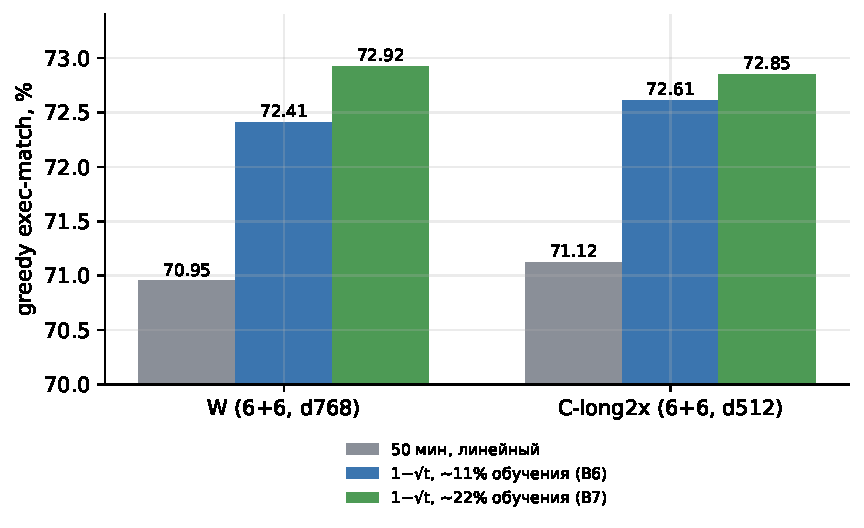
\includegraphics[width=.62\linewidth]{cooldown}
  \vspace{-.6em}
  \caption{Длина охлаждения. Те же стартовые веса (конец основного обучения B5), разный финальный участок.}
  \label{fig:cooldown}
\end{figure}

\subsection{Ансамбли и честная проверка}
С каждой новой моделью мы обновляли ансамбль (рис.~\ref{fig:lb}): v8~--- добавили модель W (78,5\%), v9~--- модели после B5 (78,4\%), v10~--- модели после B6 (79,0\%), v11~--- больше сэмплов на спорных задачах (79,4\%).

Отдельно мы проверили разные способы объединять модели (рис.~\ref{fig:ideas}). Для этого один раз собрали большой пул: по 16--24 сэмпла от каждой модели на 4096 задачах валидации, со всеми исполнениями. На этом пуле можно было бесплатно проверить любую политику: выбор~--- на одной половине (tune), подтверждение~--- на другой (eval) (\file{work/notes/e1-ensembles.md}, \texttt{e2-policy.md}, \texttt{tta-experiment.md}). Что пробовали, простыми словами:
\begin{itemize}
  \item \textbf{ансамбль на уровне токенов}: три модели генерируют один ответ вместе, на каждом шаге усредняя вероятности токенов; одна такая генерация хуже голосования по многим разным ответам ($-2,3$\,\pp);
  \item \textbf{перекрёстная оценка}: каждый кандидат оценивается всеми тремя моделями, и голос взвешивается этой оценкой (+0,15, шум);
  \item \textbf{model soup}: усреднить веса двух родственных моделей C в одну ($-0,05$);
  \item \textbf{смесь температур}: часть сэмплов при $T=1{,}0$ ради разнообразия (+0,7, но на грани шума);
  \item \textbf{test-time augmentation}: подать вопрос в нескольких равнозначных формах (\$5 → 5 dollars), но такое правило меняет только 22\% вопросов ($-0,05$);
  \item \textbf{больше сэмплов на спорных задачах} (1/8/8 вместо 1/5/6): \textbf{+0,73\,\pp}~--- единственное, что подтвердилось.
\end{itemize}

\begin{figure}[h]
  \centering
  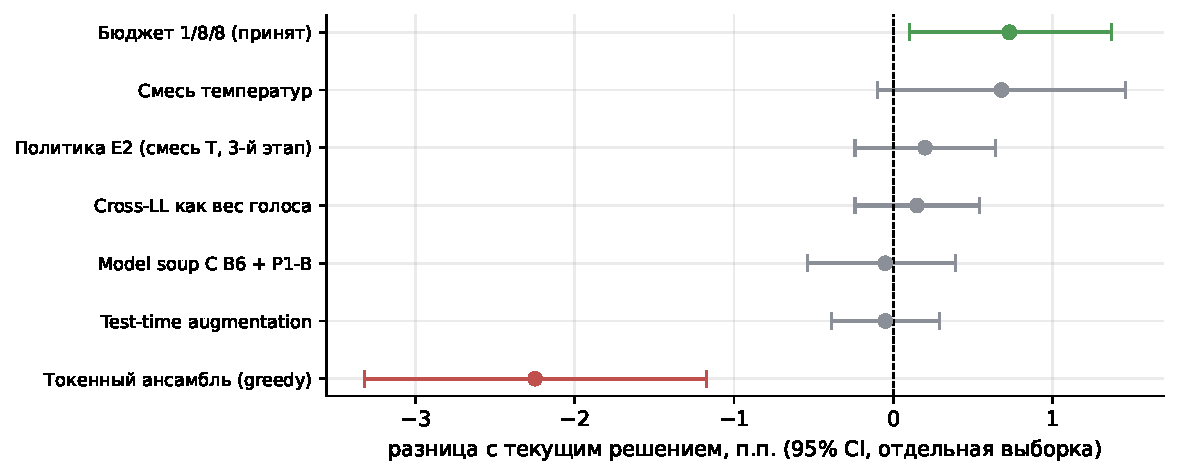
\includegraphics[width=.75\linewidth]{ideas}
  \vspace{-.8em}
  \caption{Идеи для инференса, проверенные на отдельной выборке. Зелёный~--- прирост подтверждён, красный~--- вредит.}
  \label{fig:ideas}
\end{figure}

В конце мы перебрали все 120 троек из 10 сохранённых моделей. Оказалось, что десятки троек дают одинаковое качество в пределах шума, и P1-B ничем не особенна. Пять лучших вариантов мы отправили в бота (табл.~\ref{tab:variants}, \file{work/notes/final-variants.md}). Все они оказались лучше v11 на public, а между собой в пределах шума. Финальным выбрали v2: у него лучший результат и на свежем tune, и на public, и он самый быстрый.

\begin{table}[h]
\centering\small
\caption{Финальные варианты ансамбля. Первая модель~--- якорь (greedy).}
\label{tab:variants}
\begin{tabular}{llccc}
\toprule
& Состав & Время, с & Tune, из 2048 & Public, \% \\
\midrule
v11 & C B6 + P1-B + W B6 & 127 & 1547 & 79,37 \\
v1 & W B7 + C B7 + W B6 & 132 & 1552 & 80,00 \\
\textbf{v2 (финал)} & \textbf{W B7 + C B7 + P1-B} & \textbf{111} & \textbf{1557} & \textbf{80,10} \\
v3 & C B6 + P1-B + W B7 & 116 & 1552 & 79,90 \\
v4 & v11 + политика E2 & 151 & 1548 & 79,90 \\
v5 & C B6 + W B6 + C B7 & 111 & 1548 & 80,10 \\
\bottomrule
\end{tabular}
\end{table}

\subsection{Что не сработало}
\begin{center}\small
\begin{tabularx}{\linewidth}{l>{\raggedright\arraybackslash}Xr}
\toprule
Идея & Что произошло & Эффект \\
\midrule
Loss truncation в основном обучении (B4) & отбрасывали 10\% «трудных» примеров в каждом батче & $-0,95$\,\pp \\
Фильтр шумных пар (D1) & модели плохо находят ошибки в разметке: точность 14\% & не применили \\
Глубокий энкодер 12 слоёв (R1) & рост «с сохранением функции» & $+0,15$ (шум) \\
Модель-ревьюер (код\,→\,вопрос) & переранжирование кандидатов & 0 \\
Продолжение обучения без длинного охлаждения (B5) & +9 ч обучения & $+0,05$ / $-0,24$ \\
Test-time augmentation & варианты записи вопроса (\$5 → 5 dollars) & $-0,05$ \\
Токенный ансамбль, model soup, cross-LL & другие способы объединить модели & $-2,25$\,…\,$+0,15$ \\
Greedy всех трёх моделей как голоса & голоса похожи и перевешивают сэмплы & $-0,6$\,…\,$-0,9$ \\
\bottomrule
\end{tabularx}
\end{center}

\subsection{Сколько вычислений ушло}
Весь этап 2 шёл на Kaggle (2$\times$T4). На рис.~\ref{fig:compute} все GPU-сессии этого этапа: длинные обучения по 4--11 часов, разведочные S1--S3 и около 40 коротких запусков (смоуки перед каждым длинным обучением, прогоны инференса, сбор пула E1, TTA, финальные варианты). Всего около 118 часов. Для L1 показано только основное обучение, а короткие запуски~--- оценка по сумме. Эксперименты этапа 1 шли в Colab на маленьких моделях и сюда не входят.

\begin{figure}[h]
  \centering
  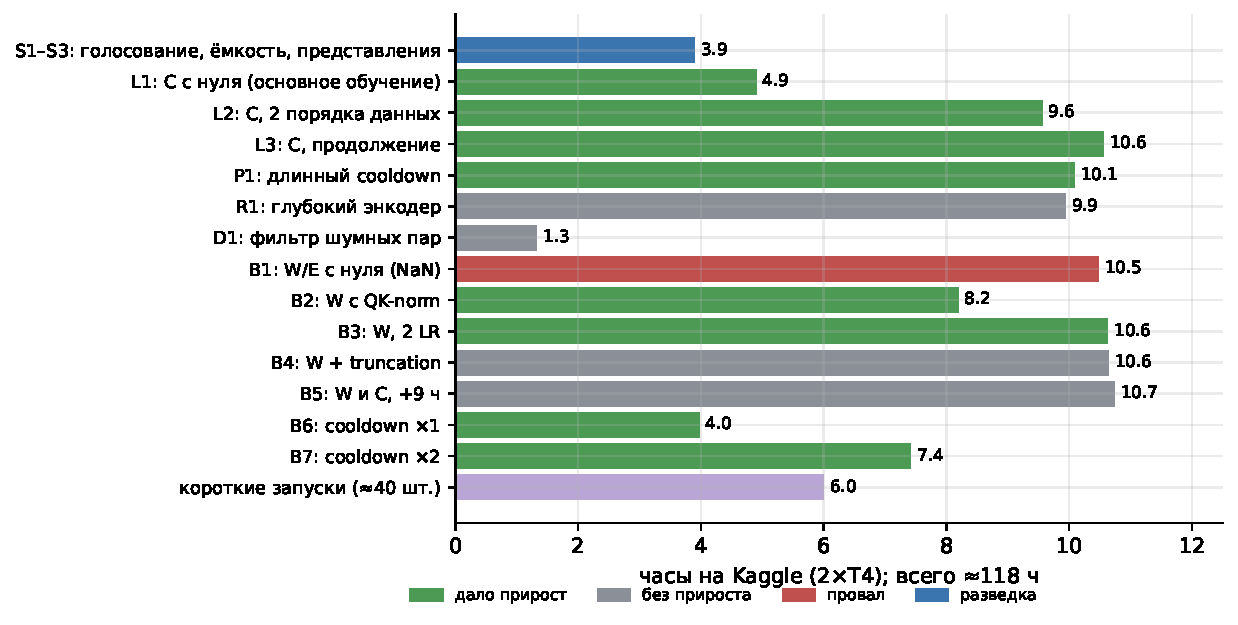
\includegraphics[width=.7\linewidth]{compute}
  \vspace{-.6em}
  \caption{GPU-сессии этапа 2 на Kaggle и их итог.}
  \label{fig:compute}
\end{figure}

%======================================================================
\section{Выводы}
\begin{itemize}
  \item Маленькая модель с правильным рецептом решает $\approx$73\% задач сама и $\approx$80\% с голосованием по исполнению.
  \item Самые полезные решения~--- не архитектурные трюки, а «скучные» вещи: правильная метрика, скорость обучения, нормировка эмбеддингов, расписание LR и длинное охлаждение.
  \item Голосование быстро насыщается; дальше помогают только более сильные модели.
\end{itemize}

%======================================================================
\section*{Где что лежит}
\small
Репозиторий: \repo. Пути~--- относительно его корня.

\begin{center}
\begin{tabularx}{\linewidth}{>{\raggedright\arraybackslash}p{.42\linewidth}>{\raggedright\arraybackslash}X}
\toprule
Путь & Что там \\
\midrule
\file{submission/inference.ipynb} & финальный ноутбук: генерирует ответы для теста на одной T4 \\
\file{submission/README.md} & как запустить (Kaggle и Colab), веса, проверки \\
\file{submission/code/hw2_codegen/} & чистый код: модель, токенизатор, декодер, исполнение, голосование, обучение \\
\file{submission/report/} & этот отчёт (LaTeX и графики) \\
\href{\repourl/tree/main/work/notebooks}{\path{work/notebooks/01-*.ipynb}}~…~\texttt{26b-*} & эксперименты этапа 1 \\
\file{work/notes/} & план, ревью и результаты каждого эксперимента \\
\file{work/kaggle/} & сборщики и код запусков этапа 2 на Kaggle \\
\file{work/research/} & скрипты анализа результатов \\
\file{work/results/} & итоговые метрики и таблицы (JSON, CSV, графики) \\
\file{work/submissions/} & все отправленные в бота файлы ответов \\
\bottomrule
\end{tabularx}
\end{center}

Веса финальных моделей~--- публичный Kaggle-датасет \href{\weightsurl}{\texttt{thisarivson/nlp-hw02-final-weights}}, версия~4: три FP16-файла весов, токенизатор, копия пакета \path{hw2_codegen} и входы теста. Как его подключить~--- в \file{submission/README.md}.

\end{document}
